
\newpage
\section{Analisi dei rischi} \label{AnalisiDeiRischi}
	Per svolgere il progetto in maniera efficiente ed efficace, viene effettuata un'analisi preliminare dei rischi che possono ostacolare il processo di sviluppo.
	È quindi fondamentale avere un sistema che ne permetta la gestione per poter agire immediatamente e con un piano ben definito in caso dovessero presentarsi.\\
	I seguenti punti rappresentano come è stato deciso di trattare i rischi:
	\begin{itemize}
		\item Identificazione: individuare i potenziali rischi che possono presentarsi
		\item Analisi: determinarne la probabilità di occorrenza e comprenderne la criticità
		\item Pianificazione: definire strategie che possono evitare i rischi precendentemente trovati
		\item Controllo: si monitorano e revisionano i rischi finche nel corso del progetto
		\item Revisione: in caso dovessero presentarsi, dopo averli risolti, si rivede la strategia utilizzata e in caso ci siano migliorie possibili si rivede (e in caso non fosse stata definita una strategia per tale rischio se ne definisce una)
	\end{itemize}
	\subsection{Valutazione}
	Per la valutazione dei rischi viene utilizzato uno strumento di misura chiamato qualitative risk assessment, che ne considera i criteri quantitativi e qualitativi assegnando a ciascuno un valore di gravità determinato dalla probabilità che possa avvenire e dalla gravità che pone al progetto.
	% VEDI : https://www2.deloitte.com/content/dam/Deloitte/it/Documents/risk/Board%20Academy%20Corso%20C6%2020%20dic%202012%20SDA%20Bocconi.pdf
	Dato il numero non elevato di rischi, si è scelto di mettere solamente tre livelli di gravità e probabilità producendo quindi una matrice con nove elementi in grado assegnare classi con valori basso, medio o alto.
	\begin{figure}[H]
		\centering
		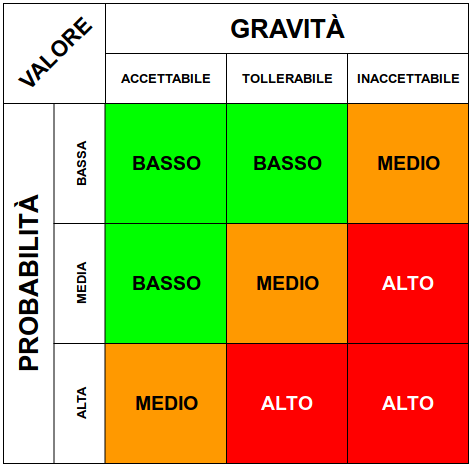
\includegraphics[scale=0.6]{img/risk_assessment_table.png}\\
		\caption{Matrice del qualitative risk assessment}
	\end{figure}
	\subsection{Tipologia}
	Le tipologie in cui suddividere i rischi sono state prese dal libro Software Engineering\footnote{10° edizione, Pagina 648, Capitolo 22: Project management} e sono:
	\begin{itemize}
 		\item \textbf{Organizzativo}: dovuto alla gestione di persone che hanno diverse responsabilità all'interno progetto.
		\item \textbf{Personale}: riguarda le conoscenze, i tempi e la formazione personali.
		\item \textbf{Requisiti}: ha a che fare con il grande numero di requisiti.
		\item \textbf{Strumentale}: per la performance degli strumenti.
		\item \textbf{Tecnologico}: per guasti nelle tecnologie.
	\end{itemize}
	\subsection{Classificazione}
	A ciascun rischio viene assegnato un codice identificativo in modo da essere facilmente riconoscibile e da comprenderne le generalità (come classe, probabilità e severità) senza andare a cercarle nelle tabelle che comprendono tutti i rischi del progetto analizzati.
	Questo codice è composto da:
	\begin{itemize}
		\item Iniziale della tipologia (O, P, R, S, T)
		\item Numero progressivo di due cifre (00 - 99)
		\item Valore di gravità (0 - Accettabile, 1 - Tollerabile, 2 - Inaccettabile)
		\item Valore di probabilità (0 - Bassa, 1 - Media, 2 - Alta)
		\item Valore della classe (0 - Basso, 1 - Medio, 2 - Alto)
	\end{itemize}
	Ad esempio da un codice come P01-021 si può immediatamente capire, sapendo cosa rappresenta ciascun simbolo, che è si tratta di un rischio del personale, con un numero progressivo 01, di gravità accettabile, probabilità alta e un valore di classe medio
	
	\subsection{Lista rischi possibili}
	Per elencare i rischi viene la seguente struttura tabellare:
	\begin{table}[H]
		\begin{risktable}{\columnwidth}{m{1.5cm}m{11.7cm}}
			\thead{ID} & 
			\thead{Nome significativo}\\
			\hline
			\rowcolor{gray!15}
			\multicolumn{2}{X}{
				\thead{Breve descrizione}
			}\\
			\hline
			\multicolumn{2}{X}{
				\thead{Strategie per la rilevazione}
			}\\
			\hline
			\rowcolor{gray!15}
			\multicolumn{2}{X}{
				\thead{Contromisure e mitigazione}
			}\\
		\end{risktable}
		\caption{Struttura tabella analisi rischio}
	\end{table}

	\noindent
	Dopo un'attenta analisi del capitolato e dopo alcuni incontri da parte dei componenti del gruppo, è stato deciso di catalogare i seguenti rischi, elencati in maniera crescente rispetto all'ID:\\
	
	\mydoublerule{\linewidth}{0pt}{2pt}
	
	\begin{table}[H]
		\begin{risktable}{\columnwidth}{m{1.5cm}m{13.5cm}}
			\thead{P00-111} & 
			Inesperienza del team a livello tecnico\\
			\hline
			\rowcolor{gray!15}
			\multicolumn{2}{X}{
				Non tutti i componenti del gruppo hanno le conoscenze di ambienti di sviluppo, linguaggi di programmazione e strumenti richiesti dall'azienda allo stesso livello.
			}\\
			\hline
			\multicolumn{2}{X}{
				Sarà compito del responsabile di progetto parlare con il resto del gruppo e capire ciascuno che conoscenze ha delle tecnologie da utilizzare per sviluppare il progetto.
			}\\
			\hline
			\rowcolor{gray!15}
			\multicolumn{2}{X}{
				Ciascun componente si impegna a sanare le proprie lacune e portarsi ad un livello comune concordato in modo da poter lavorare autonomamente e potersi prendere impegni risolvibili senza dover usare tempo ulteriore per imparare la tecnologia.
			}\\
		\end{risktable}
	\end{table}

	\mydoublerule{\linewidth}{0pt}{2pt}

	\begin{table}[H]
		\begin{risktable}{\columnwidth}{m{1.5cm}m{13.5cm}}
			\thead{P01-122} & 
			Impreparazione del team a livello gestionale \\
			\hline
			\rowcolor{gray!15}
			\multicolumn{2}{X}{
				Non avendo affrontato progetti del genere prima d'ora, i componenti del gruppo non conoscono bene i ruoli che devono intraprendere e i compiti da svolgere.				
			}\\
			\hline
			\multicolumn{2}{X}{
				Sarà compito del componente che fa da responsabile assicurarsi che non ci siano perplessità da parte degli altri membri sui ruoli ricoperti e sui compiti che assegnati.
			}\\
			\hline
			\rowcolor{gray!15}
			\multicolumn{2}{X}{
				Durante le ore di studio personale, ciascun componente si impegna a studiare la gerarchia dei ruoli\footnote{Consultabile nel materiale fornito dal professore e sul libro di testo Software Engineering}, in caso di dubbi ne potrà parlare con il gruppo oppure direttamente con chi fa da responsabile.
			}\\
		\end{risktable}
	\end{table}
	
	\mydoublerule{\linewidth}{0pt}{2pt}
		
	\begin{table}[H]
		%TODO rivedere
		\begin{risktable}{\columnwidth}{m{1.5cm}m{13.5cm}}
			\rowcolor{red}			
			\thead{O00-201} & 
			Ritardo consegna del materiale per una revisione oltre la scadenza \\
			\hline
			\rowcolor{gray!15}
			\multicolumn{2}{X}{
				È possibile che uno o più componenti del gruppo non riescano a gestire i compiti assegnati e quindi arrivare a una scadenza senza aver finito il proprio lavoro, obbligando l'intero gruppo rinviare la consegna.
			}\\
			\hline
			\multicolumn{2}{X}{
				Sarà compito del responsabile assicurarsi che il lavoro proceda in maniera lineare ponendo scadenze intermedie, monitorando il lavoro del gruppo, organizzando riunioni e aggiornandosi sullo stato dei vari compiti assegnati secondo il way of working scelto.
			}\\
			\hline
			\rowcolor{gray!15}			
			\multicolumn{2}{X}{
				Ciascun membro si impegna a gestire il proprio tempo adeguatamente in rapporto con gli altri impegni universitari senza tralasciare il suo ruolo nello sviluppo del progetto. In caso di impegni che possano ostacolare ciò, si prenderà cura di avvisare gli altri componenti del gruppo per tempo.
			}\\
		\end{risktable}
	\end{table}
	
	\mydoublerule{\linewidth}{0pt}{2pt}
	
	\begin{table}[H]
		\begin{risktable}{\columnwidth}{m{1.5cm}m{13.5cm}}
			\thead{P02-100} & 
			Approvazione errata di documenti \\
			\hline
			\rowcolor{gray!15}
			\multicolumn{2}{X}{
				È possibile che il responsabile commetta errori nella fase di approvazione dei documenti che possono portare alla consegna di documentazione errata o fatta male, causando quindi disguidi con il cliente (oltre a lasciare un'impressione negativa) e necessità di rivedere tali sviste, andando quindi a sprecare risorse investibili in altri compiti.
			}\\
			\hline
			\multicolumn{2}{X}{
				%TODO: rivedere
				Colui che svolge il ruolo di responsabile deve avere modo di controllare il lavoro prodotto dal proprio team in modo costante e graduale.
			}\\
			\hline
			\rowcolor{gray!15}
			\multicolumn{2}{X}{
				Chi al momento svolge il ruolo di responsabile deve assicurarsi che i documenti approvati siano effettivamente validi e in caso di sviste il verificatore deve saper trovare e correggere gli eventuali errori.
			}\\
		\end{risktable}
	\end{table}
	
	\mydoublerule{\linewidth}{0pt}{2pt}
	
	\begin{table}[H]
		
		\begin{risktable}{\columnwidth}{m{1.5cm}m{13.5cm}}
			\thead{P03-100} & 
			Cattiva gestione dell'archivio di documentazione di progetto\\
			\hline
			\rowcolor{gray!15}			
			\multicolumn{2}{X}{
				Data la poca esperienza dei componenti del gruppo con progetti di questo genere dove la documentazione è una delle parti principali, gestirla può risultare una cosa nuova e potrebbe presentare difficoltà.
			}\\
			\hline
			\multicolumn{2}{X}{
				L'amministratore deve aver predisposto una repository comune in cui ciascun componente potrà caricare il proprio lavoro e dovrà saperla utilizzare in maniera tale da non andare a modificare quel che è stato caricato dagli altri.
			}\\
			\hline
			\rowcolor{gray!15}			
			\multicolumn{2}{X}{
				In caso di erorri di gestione della repository l'amministratore deve saperli risolvere in maniera tempestiva in modo da evitare che chi la andrà ad utilizzare successivamente scarichi file errati e di conseguenza vada a propagare l'errore anche sul proprio sistema.
			}\\
		\end{risktable}
		
	\end{table}

	\mydoublerule{\linewidth}{0pt}{2pt}
	
	\begin{table}[H]
		%TODO rivedere
		\begin{risktable}{\columnwidth}{m{1.5cm}m{13.5cm}}
			\rowcolor{red}			
			\thead{P04-021} & 
			Non conoscenza totale o parziale tra i membri\\
			\hline
			\rowcolor{gray!15}
			\multicolumn{2}{X}{
				Il gruppo è formato principalmente da persone che precedentemente non si conoscevano o che hanno avuto poche interazioni fra di loro fino al momento della creazione di quest'ultimo. Ciò può comportare una cattiva gestione del lavoro e dell'assegnazione dei compiti, poiché non si conoscono le competenze altrui.
			}\\
			\hline
			\multicolumn{2}{X}{
				Tra incontri faccia a faccia e strumenti di comunicazione quali chat su Telegram o Slack, ci si confronta e si realizzano i diversi modi di lavorare di ognuno.
			}\\
			\hline
			\rowcolor{gray!15}
			\multicolumn{2}{X}{
				Il gruppo si impegna a conoscersi nel corso delle riunioni e ritrovi. Si discute inoltre insieme di un way of working comune che possa soddisfare le metodologie di lavoro di tutti i componenti.
				È possibile che ci siano dibattiti e non ci si riesca a mettere d'accordo su argomenti vari; in questo caso vince l'opinione della maggioranza.
				%In caso ci fossero dibattiti, per non ricorrere alle lame, gli altri componenti andranno a calmare le acque senza che ci siano morti.
				%LOOOL
			}\\
		\end{risktable}
		
	\end{table}
	
	%TODO LAURA: COINCIDE CON Ritardo consegna del materiale per una revisione oltre la scadenza 
	\mydoublerule{\linewidth}{0pt}{2pt}
	\begin{table}[H]
		\begin{risktable}{\columnwidth}{m{1.5cm}m{13.5cm}}
			\rowcolor{red}
			\thead{X00-000} & 
			Impegni personali e universitari da gestire in parallelo al progetto \\
			\hline
			\rowcolor{gray!15}			
			\multicolumn{2}{X}{
				Ciascun membro ha impegni legati alla propria vita privata e all'università, è possibile quindi che possano insorgere indisponibilità di tempo da dedicare al progetto.
			}\\
			\hline
			\multicolumn{2}{X}{
				Sarà compito del responsabile fissare gli incontri e la spartizione del lavoro coordinandosi con gli altri membri in modo tale da assicurare la buona collaborazione di ciascun membro equamente, e questi ultimi devono riuscire a distinguere le priorità in modo da non influenzare negativamente lo sviluppo del progetto.
			}\\
			\rowcolor{gray!15}
			\hline
			\multicolumn{2}{X}{
				In caso di indisposizione ci dovrà essere una giustificazione data per tempo valutando inoltre che conseguenze può avere sulla redistribuzione del lavoro e delle risorse sapendo.
			}\\
		
		\end{risktable}
	\end{table}
	
	\mydoublerule{\linewidth}{0pt}{2pt}
	
	\begin{table}[H]
		\begin{risktable}{\columnwidth}{m{1.5cm}m{13.5cm}}
			\thead{S00-100} & 
			Problematiche hardware \\
			\hline
			\rowcolor{gray!15}			
			\multicolumn{2}{X}{
				È possibile che i computer e altri strumenti hardware che possono essere utilizzati dai membri del gruppo possano difettarsi e smettere di funzionare.
			}\\
			\hline
			\multicolumn{2}{X}{
				%TODO LAURA: da mettere in mitigazione?
				Ciascun membro avrà cura degli strumenti a sua disposizione in modo tale che non sorgano problemi che possano ostacolare il proprio lavoro.
			}\\
			\hline
			\rowcolor{gray!15}			
			\multicolumn{2}{X}{
				I guasti di natura hardware non sono facilmente prevedibili e in caso dovesse succedere è possibile utilizzare temporaneamente i computer forniti dai laboratori dell'università fino a quando non si ripara, o se necessario sostituisce, la propria macchina.
			}\\
		\end{risktable}
	\end{table}
	
	\mydoublerule{\linewidth}{0pt}{2pt}
	
	\begin{table}[H]
		
		\begin{risktable}{\columnwidth}{m{1.5cm}m{13.5cm}}
			\rowcolor{red}
			\thead{R00-122} & 
			Aggiunta o modifica di requisiti in corso di sviluppo \\
			\hline
			\rowcolor{gray!15}
			\multicolumn{2}{X}{
				Durante il progetto, dopo aver effettuato una prima analisi di tutti i requisiti, può nascere il bisogno di modificare un requisito già fissato o aggiungerne uno non identificato in precedenza.
			}\\
			\hline
			\multicolumn{2}{X}{
				È possibile che nel corso dello sviluppo del progetto vengano scoperti requisiti secondari impliciti non precedentemente valutati che necessitano di essere sviluppati.
			}\\
			\hline
			\rowcolor{gray!15}			
			\multicolumn{2}{X}{
				In caso dovessero sorgere necessità di sviluppare requisiti inaspettati, questi andranno analizzati per capire di che risorse hanno bisogno e saranno inseriti nella scaletta dello sviluppo del progetto in modo adeguato. Data la natura modulare del progetto, ciascun requisito verrà sviluppato dal più al meno importante in modo da poter avere compiti facilmente monitorabili e testati.
			}\\
		\end{risktable}
		
	\end{table}
	
	\mydoublerule{\linewidth}{0pt}{2pt}
	
	\begin{table}[H]
		
		\begin{risktable}{\columnwidth}{m{1.5cm}m{13.5cm}}
			\rowcolor{red}
			\thead{T00-100} & 
			Problematiche software\\
			\hline
			\rowcolor{gray!15}
			\multicolumn{2}{X}{
				Il gruppo fa affidamento a prodotti software per l'integrazione del codice e dei documenti. Eventuali guasti possono causare gravi perdite di dati.
			}\\
			\hline
			\multicolumn{2}{X}{
				Siccome ci si affida a servizi di terze parti, i malfunzionamenti che possono capitare sono imprevedibili, ma data la nota affidabilità di questi strumenti la probabilità che questo rischio accada è molto bassa.
			}\\
			\hline
			\rowcolor{gray!15}
			\multicolumn{2}{X}{
				Ciascun componente si impegna a mantenere una copia, aggiornata periodicamente, della repository contenente il proprio lavoro, su computer o eventualmente una memoria esterna.
			}\\
		\end{risktable}
		
	\end{table}

	\mydoublerule{\linewidth}{0pt}{2pt}
	
	%TODO LAURA: tratta le stesse cose di: Aggiunta o modifica di requisiti in corso di sviluppo 
	\begin{table}[H]
		
		\begin{risktable}{\columnwidth}{m{1.5cm}m{13.5cm}}
			\thead{X00-000} & 
			Interpretazione errata dei requisiti.\\
			\hline
			\rowcolor{gray!15}
			\multicolumn{2}{X}{
				Dato il documento contenente le specifiche richieste dall'azienda per il prodotto da sviluppare, alcuni requisiti possono essere mal interpretati.
			}\\
			\hline
			\multicolumn{2}{X}{
				A ciascuna milestone, anche intermedia, è utile controllare che la lista dei requisiti da svolgere sia coerente con quelli richiesti dall'azienda nel documento che presenta il loro capitolato.
				Sarà compito del responsabile che il progetto avanzi completando in modo graduale tutti i requisiti richiesti dall'azienda.
			}\\
			\hline
			\rowcolor{gray!15}
			\multicolumn{2}{X}{
				In caso dovessero sorgere problemi sull'implementazione errata di un requisito, questo verrà fuori alla prossima riunione in cui si discute dei progressi di ciascun componente e in caso ci fossero dubbi, questi verranno discussi con il resto del gruppo e se necessario con i rappresentanti dell'azienda.
			}\\
		\end{risktable}
		
	\end{table}
	
	\mydoublerule{\linewidth}{0pt}{2pt}

	\begin{table}[H]
		%rischio organizzativo?!
		\begin{risktable}{\columnwidth}{m{1.5cm}m{13.5cm}}
			\thead{O01-010} & 
			Mancanza di comunicazione con l'azienda \\
			\hline
			\rowcolor{gray!15}
			\multicolumn{2}{X}{
				 Durante lo sviluppo del progetto è possibile che il gruppo non contatti i rappresentanti dell'azienda e che questi quindi non siano al corrente dei progressi fatti, dei requisiti completati e del modo in cui si è lavorato.
			}\\
			\hline
			\multicolumn{2}{X}{
				È opportuno che il responsabile si metta in comunicazione con l'azienda (Telegram, Skype on incontri di persona) e riferisca il progresso svolto dal gruppo in modo da avere feedback e critiche costruttive che possano migliorare lo sviluppo successivo.
			}\\
			\hline
			\rowcolor{gray!15}			
			\multicolumn{2}{X}{
				In caso di mancata comunicazione per un lungo arco di tempo è opportuno che alla prima scadenza di revisione utile posta dal professore il gruppo si impegni a contattare l'azienda per avere un suo feedback.
			}\\
		\end{risktable}
		
	\end{table} 	

	\mydoublerule{\linewidth}{0pt}{2pt}
	
	\begin{table}[H]
		
		\begin{risktable}{\columnwidth}{m{1.5cm}m{13.5cm}}
			\thead{P05-122} & 
			Cattiva amministrazione delle risorse \\
			\hline
			\rowcolor{gray!15}
			\multicolumn{2}{X}{
				Data l'inesperienza del gruppo con progetti di questa natura è possibile che ci sorgano errori nell'amministrazione delle risorse come tempo, costi e suddivisione persone / ruoli.
			}\\
			\hline
			\multicolumn{2}{X}{
				A ciascun incontro con il gruppo si controllerà se il lavoro svolto finora è pertinente a quanto è stato preventivato modificando di conseguenza il consuntivo e il preventivo a finire.
				Tramite strumenti come diagrammi di Gantt dinamici (dove ciascun componente può aggiornare i tempi previsiti per completare l'attività assegnata) è possibile monitorare costantemente il progresso del progetto in modo tale da evitare situazioni di zero laxity.
			}\\
			\hline
			\rowcolor{gray!15}			
			\multicolumn{2}{X}{
				In caso dovessero sorgere problemi di questa natura il gruppo si impegnerà a ridistribuire le risorse in modo da arrivare corretti alla prossima consegna posta dal professore tenendo conto di consegnare comunque un lavoro di qualità.
			}\\
		\end{risktable}
		
	\end{table} 

	\mydoublerule{\linewidth}{0pt}{2pt}